%%%%%%%%%%%%%%%%%%%%%%%%%%%%%%%%%%%%%%%%%%%%%%%%%%%%%%%%%%%%%%%%%%%%%%%%%%%%%%%%
% SII 2027 regular paper -- 4-6 pages; up to 8 pages with extra-page charges.
% Main file MUST remain root.tex for PaperPlaza's TeX -> PDF conversion.
% Figure-generation source and statistics should accompany the final archive.
%%%%%%%%%%%%%%%%%%%%%%%%%%%%%%%%%%%%%%%%%%%%%%%%%%%%%%%%%%%%%%%%%%%%%%%%%%%%%%%%

% cmd: latexmk -pdf -interaction=nonstopmode -halt-on-error root.tex

\documentclass[a4paper, 10pt, conference]{ieeeconf}

\IEEEoverridecommandlockouts
\overrideIEEEmargins

\usepackage{graphicx}
\usepackage{amsmath}
\usepackage{amssymb}
\usepackage{booktabs}
\usepackage{tikz}
\usepackage{xcolor}
\usetikzlibrary{arrows.meta,positioning,calc}

\graphicspath{{figures/}}

% Notation follows the RIL manuscript: lowercase symbols are single-sample row
% vectors, uppercase symbols are matrices of stacked samples.
\newcommand{\vB}{v_B}
\newcommand{\vj}{v_j}
\newcommand{\Jm}{J}
% Revision markup for internal review: original text is red and revised text is
% blue (now in black). Remove the red text and blue coloring before submission.
\newcommand{\oldtext}[1]{\textcolor{red}{}}
\newcommand{\newtext}[1]{\textcolor{black}{#1}}

\title{\LARGE \bf
\newtext{Online Rapid Innate Learning via Recursive Least-Squares \\
for Online Legged Locomotion Learning}
}

\author{
  Julathit Chetsawang$^{1}$,
  Warit Yuvaniyama$^{1}$,
  Krittapak Jairak$^{1}$,\\
  Kaweewat Sricharoenchit$^{1}$,
  Bing Gwong Leung$^{1}$,
  Yasushi Mae$^{2}$,
  Photchara Ratsamee$^{2}$
\thanks{$^{1}$Julathit Chetsawang, Warit Yuvaniyama, Krittapak Jairak, Kaweewat Sricharoenchit, and Bing Gwong Leung are with the School of Information, Computer, and Communication Technology (ICT), Sirindhorn International Institute of Technology (SIIT), Thammasat University, Pathum Thani 12120, Thailand
{\tt\small \{6622782280, 6622770459, 6622782207, 6622782181\}@g.siit.tu.ac.th},
{\tt\small bile@siit.tu.ac.th}}%
\thanks{$^{2}$Yasushi Mae and Photchara Ratsamee are with the Department of Mechanical Engineering, Graduate School of Science and Engineering, Kansai University, Suita, Osaka, Japan
        {\tt\small \{mae, ratsamee\}@kansai-u.ac.jp}}%
}

\begin{document}

\maketitle
\thispagestyle{empty}
\pagestyle{empty}

%%%%%%%%%%%%%%%%%%%%%%%%%%%%%%%%%%%%%%%%%%%%%%%%%%%%%%%%%%%%%%%%%%%%%%%%%%%%%%%%
\begin{abstract}
% \oldtext{Rapid innate learning (RIL) enables a legged robot to acquire a walking
% gait within seconds by combining joint-torque contribution learning with motor
% babbling, producing a per-leg weight matrix derived from the map between joint
% velocity and body velocity, which modulates a central pattern generator. That
% matrix is estimated once, from babbling performed with the feet planted, so it
% describes the robot before it walks rather than while it walks. The mismatch is
% not uniform across legs, and the resulting per-leg bias makes each run travel in
% a different direction. This paper proposes online recursive refinement to
% address this mismatch: the batch estimate seeds a recursive least-squares
% estimator that continues to track the map at the control rate during locomotion,
% with a stop-learning mechanism that suspends adaptation when the joints carry no
% information. Evaluated in simulation on a four-legged robot, refinement reduces
% absolute heading error from $26.3^\circ$ to $5.5^\circ$ and lateral drift from
% $1.02$\,m to $0.25$\,m at unchanged forward speed, and reduces run-to-run spread
% by roughly a factor of four. We report the refinement in simulation only.
% Separately, as a feasibility study of the underlying batch mechanism, we deploy
% RIL without refinement on a Unitree Go2 quadruped through a $500$\,Hz low-level
% joint interface, where the robot re-runs the identification on its own hardware
% and walks in three commanded directions. That study makes no claim about the
% online estimator, which remains to be validated on hardware.}

\newtext{Motivated by fawns and other precocial mammals—animals that can stand and walk just hours after birth
without prior training—we incorporated an online Recursive Least Squares (RLS) method into Rapid Innate Learning (RIL).
This enables learning, during a short motor-babbling period, a morphology-specific mapping from joint velocity to body linear velocity;
the resulting controller weights then shape a central pattern generator.
Because baseline RIL is carried out with the robot standing still and its feet fixed on the ground,
the resulting static map may fail to capture the contact-dependent effects present during locomotion,
which can cause trial-to-trial variability in travel direction. To address this, we extend RIL with an exponentially weighted RLS scheme
that continuously updates each leg's horizontal velocity map as the robot walks.
A batch solution is used to initialize the recursion, and update mechanisms such as joint-motion gating and
covariance bounding constrain learning during intervals that provide little useful information.
Across $100$ simulation runs per condition, online refinement reduced mean absolute heading error from
$26.3^\circ$ to $5.5^\circ$ and mean absolute lateral drift from $1.02$\,m to
$0.25$\,m. Mean forward speed remained comparable ($0.263$ versus
$0.253$\,m/s), and gait failures decreased from five runs to none. In a separate
hardware feasibility study, we deployed RIL,
without online refinement, on a Unitree Go2 through a $500$\,Hz low-level joint
interface. The robot identified its controller weights from its own measurements
and responded to forward, backward, and in-place commands. These results provide
simulation evidence for Online RLS in RIL and establish the hardware feasibility of the
underlying RIL pipeline.}
\end{abstract}

%%%%%%%%%%%%%%%%%%%%%%%%%%%%%%%%%%%%%%%%%%%%%%%%%%%%%%%%%%%%%%%%%%%%%%%%%%%%%%%%
\section{INTRODUCTION}
\label{sec:intro}

% \oldtext{Enabling a legged robot to walk without hand-designing its gait is
% normally treated as a learning problem, and solving it requires experience. Deep
% reinforcement learning produces quadruped controllers
% \cite{hwangbo2019,lee2020}, but only after large numbers of simulated trials and a
% transfer stage before the policy reaches hardware. Central pattern generators
% (CPGs) occupy the other extreme \cite{ijspeert2008,miguelblanco2020}: they are
% compact, inherently rhythmic, and cheap to evaluate. A CPG does not supply the
% mapping from oscillator output to individual joint commands. That mapping encodes
% the morphology of the robot, and a designer must otherwise write it by hand for
% each new body. Changing the leg geometry, the mass distribution or the number of
% legs means rewriting the mapping again.}

\newtext{Learning legged locomotion is a challenging problem due to the coordination of its joints to maintain balance and generate desired body motion under
nonlinear and intermittent contact. Among the approaches developed to address
this challenge, deep reinforcement learning has produced highly capable
controllers. These controllers are typically trained through millions of
simulated interactions, often distributed across thousands of GPU-parallel robot
instances, before being transferred to hardware
\cite{hwangbo2019,lee2020,rudin2022,makoviychuk2021}. Their performance therefore
comes at the cost of substantial training experience and computational
resources.}

% \oldtext{Newborn animals must solve the same problem, and they do so without a
% training period or a hand-designed mapping. Stick insects walk immediately after
% hatching \cite{zeng2020}, and precocial mammals walk within minutes to a few
% hours of birth \cite{garwicz2009,vandenhole2017}, across large differences in
% body size, morphology and limb configuration. Locomotion appears without a
% rehearsal period, on a body the animal has not controlled before. Reproducing that
% capability on a robot would remove the need to re-engineer the controller for
% each new robot body. Rapid innate learning (RIL) \cite{leung2023,ril} adopts that
% premise for robots and produces the missing mapping automatically, in seconds and
% without a walking trial. Joint-torque contribution learning measures, while the
% robot stands, the share of the supporting load carried by each joint, which
% governs vertical leg motion \cite{leung2023}. Motor babbling then moves the
% joints randomly, one at a time, and regresses the observed body velocity on the
% measured joint velocities to obtain the horizontal contribution of each joint.
% Together the two yield a per-leg weight matrix that modulates the CPG, and
% mechanical coupling through the body lets babbling on a single active leg supply
% data for every leg \cite{ril}. No policy search is involved, and the
% identification is a single matrix solve, so the robot walks within seconds of
% start-up. Section~\ref{sec:ril} states the procedure in full, since it is the
% mechanism this paper extends.}

\newtext{By contrast, animals cannot create thousands of parallel copies of
their physical bodies, yet many species acquire locomotion rapidly from the
experience of a single individual
\cite{zeng2020,garwicz2009,vandenhole2017}. Previous work on rapid innate
learning (RIL) \cite{leung2023,ril} pursued an analogous single-robot learning
regime based on brief, robot-specific identification rather than policy
optimization. RIL combines two components. First, joint-torque contribution
learning (JTCL) estimates the vertical controller weights from joint torques
measured while the robot stands. Second, motor babbling excites the joints and
fits a horizontal joint-to-body linear-velocity map from the measured motion.
The resulting per-leg weights modulate a CPG, allowing the robot to begin walking
within seconds without a walking trial or a population of parallel learners.
RIL is therefore well suited for rapid controller initialization. However, the
map identified during babbling remains fixed throughout locomotion and cannot be
improved using subsequent walking data.}

% \oldtext{RIL identifies that matrix once, under conditions that differ from those
% in which it is used. Babbling is quasi-static: the feet stay planted, one joint
% moves at a time, and the resulting body velocity is small. During walking, in
% contrast, legs load and unload, feet make and break contact, and the body velocity
% produced by a given joint velocity depends on whether that leg is in stance. A
% linear map fitted while standing therefore describes walking only approximately.
% Because each leg is fitted from its own babbling data, the error differs between
% legs, and unequal errors make each run follow a different curve.}

\begin{figure}[t]
  \centering
  \includegraphics[width=\columnwidth]{FINALFinal_Intro_picture.jpg}
  \caption{Inspired by the motor babbling observed in fawns and other precocial mammals—animals that can rapidly coordinate their bodies, stand, and walk within hours after birth without earlier practice—we integrated an online Recursive Least Squares (RLS) method into Rapid Innate Learning (RIL). By emulating this innate exploratory behavior, the approach enables a quadruped to learn walking by quickly estimating and updating controller weights within seconds.}
  \label{fig:intro}
\end{figure}

\newtext{This limitation matters because identification and deployment occur
under different conditions (Fig.~\ref{fig:intro}). During babbling, the feet remain planted and body
motion is small. During walking, contact switches between stance and swing,
leg loading varies within each stride, and the relationship between joint velocity
and body linear velocity becomes phase dependent. A map identified while
standing can therefore produce unequal per-leg errors during locomotion, leading
to curved and run-dependent trajectories. Online adaptation methods address
related problems by updating policy inputs \cite{kumar2021}, selecting behaviors
from an offline repertoire \cite{cully2015}, or adapting CPG parameters from
sensory feedback \cite{miguelblanco2020,suzuki2019}. Recursive least
squares (RLS) is particularly suitable because the horizontal map is already
defined by a linear regression. RLS can continue that regression sample by
sample, has low computational cost, and uses the joint- and body-velocity signals
already available to the controller \cite{ljung1999,astrom1995}.}

% \oldtext{This paper updates that map while the robot walks, at negligible
% computational cost and without additional sensing, and establishes that the
% underlying mechanism runs on real hardware. The batch fit serves as an initial
% condition: the same regression continues recursively at the control rate, from
% signals the controller already reads. Recursive least squares is standard
% \cite{ljung1999,astrom1995}; the contribution is the quantity placed under
% estimation. Online methods for legged robots adapt a policy input
% \cite{kumar2021}, a gait selection \cite{cully2015}, or an oscillator parameter
% \cite{miguelblanco2020,suzuki2019}, whereas the quantity adapted here is the
% learned morphology description itself.}

\newtext{We therefore propose \emph{Online RLS in RIL}. The one-shot batch LS estimate
initializes an exponentially weighted online RLS estimator, which
updates each leg's horizontal joint-to-body velocity map at the control rate
during walking. Joint-Motion Gating skips uninformative samples, and covariance
bounding limits excessively large estimator gains. The refined map is converted
back into horizontal controller weights and used by the same distributed CPG
controller, requiring no additional sensing or policy training. The proposed
online estimator is evaluated in simulation; a separate Unitree Go2 study
evaluates only the hardware feasibility of RIL.}

% \oldtext{The two studies are validated on different platforms, so we state their
% scope separately:}
\newtext{The main contributions are as follows:}
\begin{itemize}
  % \item \oldtext{\emph{Online recursive refinement, in simulation.} We keep the
  %       RIL weight matrix under recursive least-squares estimation during
  %       locomotion, seeded by the batch solution and bounded by a stop-learning
  %       mechanism.}
  \item \newtext{\emph{Online refinement of RIL.} We develop Online RLS in RIL, an
        online learning mechanism that uses batch-initialized, exponentially
        weighted RLS to continuously refine the horizontal joint-to-body
        velocity map during locomotion. The refined map updates the horizontal
        controller weights, improving the alignment of the robot's travel
        direction with the commanded locomotion direction.}
  % \item \oldtext{\emph{Sim-to-real feasibility, on hardware.} We deploy the
  %       inherited batch mechanism on a Unitree Go2 through a $500$\,Hz low-level
  %       joint interface, without refinement.}
  \item \newtext{\emph{Quantitative simulation evaluation.} Across $100$ runs
        per controller, Online RLS in RIL reduces mean absolute heading error and
        lateral drift, eliminates the observed gait failures, and maintains
        comparable forward speed relative to RIL.}
  \item \newtext{\emph{Hardware feasibility of the underlying RIL pipeline.}
        We deploy RIL, without online refinement, on a Unitree Go2 through a
        $500$\,Hz low-level joint interface. The robot identifies its controller
        weights from physical measurements and responds to multiple commanded
        directions.}
\end{itemize}

% \oldtext{The estimator is evaluated in simulation only, and no hardware result is
% claimed for it. Because the robot re-identifies its own matrix on the physical
% platform, no fitted parameter is transferred from simulation. Running the
% estimator on hardware combines the two studies and remains future work.
% Section~\ref{sec:related} surveys related work; Section~\ref{sec:method} restates
% the inherited mechanism and the proposed refinement; Section~\ref{sec:sim}
% evaluates the refinement in simulation; and Section~\ref{sec:sim2real} reports
% the sim-to-real feasibility study. We close with limitations and conclusions.}

\newtext{The online estimator is evaluated only in simulation. The hardware study
uses RIL and therefore establishes feasibility of the underlying
identification and control pipeline rather than validation of online refinement.
The Go2 identifies its controller weights from physical measurements, so no fitted
parameter is transferred from simulation. Sections~\ref{sec:related} and \ref{sec:method}
position and define the method, Section~\ref{sec:sim} evaluates
Online RLS in RIL, and Section~\ref{sec:sim2real} reports the RIL
hardware study.}

%%%%%%%%%%%%%%%%%%%%%%%%%%%%%%%%%%%%%%%%%%%%%%%%%%%%%%%%%%%%%%%%%%%%%%%%%%%%%%%%
\section{RELATED WORK}
\label{sec:related}

\subsection{Learning-Based Locomotion Control}

Deep reinforcement learning produces quadruped controllers that remain effective over
rough and slippery terrain \cite{hwangbo2019,lee2020}, trained in massively
parallel simulation \cite{rudin2022,makoviychuk2021} and surveyed in
\cite{ha2025}. Part of this literature addresses the morphology problem directly,
e.g., with a single policy spanning quadrupeds of differing size and
kinematics \cite{shafiee2024,zargarbashi2024}.
The cost is sample complexity: training consumes millions of simulated steps
across thousands of parallel robots to yield a parameter vector fitted
to simulated dynamics, so a transfer stage of domain randomization, system
identification or fine-tuning precedes deployment. RIL occupies the opposite end
of that trade-off, running no policy search and learning from seconds of data
recorded on the physical robot, at the price of a narrower repertoire.

\subsection{Model-Based Control}

% \oldtext{Model-based controllers achieve precise and predictable behavior,
% including on difficult terrain \cite{jenelten2019}. They require a dynamic model
% of the platform together with gains identified and tuned for it, which is again
% per-morphology engineering, carried out by hand rather than by search. The map
% from joint velocity to body velocity that RIL learns is one that a model-based
% pipeline derives analytically. RIL measures it instead, which removes the
% dependence on a model but limits the estimate to the directions the robot excites
% during identification.}

\newtext{Model-based locomotion controllers compute contact forces or joint
commands from explicit rigid-body dynamics, contact constraints, and a state
estimate, commonly within an optimization or whole-body-control framework
\cite{jenelten2019}. They offer interpretable constraints and accurate tracking,
but require a sufficiently accurate robot model, inertial and contact parameters,
and platform-specific controller design. RIL does not replace such a full-order
model. Instead, it identifies a low-dimensional empirical relation between joint
velocity and body linear velocity for constructing CPG controller weights. The
quality of this learned relation is therefore determined by the excitation,
contact regime, and measurement quality during identification.}

\subsection{Bio-Inspired Locomotion Control}

Central pattern generators produce stable rhythms from very few parameters and
support decentralized, sensor-driven adaptation
\cite{ijspeert2008,miguelblanco2020,suzuki2019,szorkovszky2023}. They are compact
and degrade gracefully, but they do not supply the morphology-dependent mapping from
oscillator output to joint commands. That mapping is conventionally
hand-designed, and it must be rewritten for each new robot. RIL supplies it
automatically, and it drives the SO(2) oscillator of Section~\ref{sec:dlc}.

\subsection{Online Learning and Adaptation}

% \oldtext{Several methods adjust a legged controller while it runs. Rapid motor
% adaptation estimates a latent description of the environment online and supplies
% it to a policy trained beforehand \cite{kumar2021}. Behavior-adaptation methods
% search a repertoire computed offline to recover from damage \cite{cully2015}.
% Neural control with sensory feedback adapts oscillator parameters from
% ground-contact and load signals \cite{miguelblanco2020,suzuki2019}. Recursive
% least squares is itself a long-established tool for tracking time-varying
% parameters \cite{ljung1999,astrom1995}, and the estimator of
% Section~\ref{sec:online} is a standard instance of one. Each of these methods
% adapts a quantity that lies outside the model of the body: an input to a fixed
% policy, an index into a precomputed repertoire, or a parameter of the oscillator.
% The per-leg matrix refined here is the model of the body, which is why refining
% it corrects a directional error that those mechanisms do not address.}

\newtext{Several methods adapt a legged controller during operation. Rapid motor
adaptation estimates a latent environmental state for a pretrained policy
\cite{kumar2021}; behavior-adaptation methods select from an offline repertoire
\cite{cully2015}; and sensory feedback can adapt oscillator parameters from
contact or load measurements \cite{miguelblanco2020,suzuki2019}. RLS is a
standard method for updating linear parameter estimates online
\cite{ljung1999,astrom1995}. The distinction in this work is the estimated
quantity: rather than changing a policy input, behavior index, or oscillator
parameter, we recursively update the empirical per-leg joint-to-body velocity map
that generates RIL's horizontal controller weights.}

%%%%%%%%%%%%%%%%%%%%%%%%%%%%%%%%%%%%%%%%%%%%%%%%%%%%%%%%%%%%%%%%%%%%%%%%%%%%%%%%
% \begin{figure}[t]
%   \centering
%   \begin{tikzpicture}[
%       font=\scriptsize,
%       box/.style={draw, rounded corners=1.5pt, align=center,
%                   inner sep=2.5pt, minimum height=6.5mm, minimum width=16mm},
%       >=Stealth, line width=0.5pt
%     ]
%     \node[box] (ril) at (0,1.25)   {RIL};
%     \node[box, fill=black!8] (rls) at (2.75,1.25) {online RLS};
%     \node[box] (cpg) at (0,0)      {CPG};
%     \node[box] (ctl) at (2.75,0)   {distributed\\leg control};
%     \node[box] (rob) at (5.5,0)    {robot};

%     \draw[->] (ril) -- node[above=-0.5mm, font=\tiny] {$\Jm,\,W_v$} (rls);
%     \draw[->] (cpg) -- node[above=-0.5mm, font=\tiny] {$o_1$} (ctl);
%     \draw[->] (ctl) -- node[above=-0.5mm, font=\tiny] {$M_{(n,l)}$} (rob);
%     \draw[->] (rls.south) -- node[right=-0.3mm, font=\tiny] {$W_l$} (ctl.north);

%     \coordinate (fb) at (-1.35,-1.0);
%     \draw[->] (rob.south) |- (fb)
%       node[above right=0mm and 6mm, font=\tiny] {$\dot q,\ \tau,\ \vB$};
%     \draw (fb) -- (-1.35,2.05);
%     \draw[->] (-1.35,2.05) -| (rls.north);
%     \fill (-1.35,1.25) circle (1.1pt);
%     \draw[->] (-1.35,1.25) -- (ril.west);
%   \end{tikzpicture}
%   \caption{\oldtext{Control and learning architecture, with the signal carried on
%   each arrow. RIL identifies the weight matrix once from standing and babbling
%   data. The proposed addition (shaded) keeps the horizontal part of that matrix
%   under recursive estimation from the same feedback, and the distributed leg
%   control combines the result with the CPG phase to produce joint commands.}
%   \newtext{Overview of the Online RLS in RIL architecture. During initialization, RIL obtains
%   the vertical weights $W_v$ from standing joint torques and estimates the
%   joint-to-body linear-velocity map $J$ from motor-babbling data using batch LS.
%   Online RLS in RIL initializes the recursion with this estimate and updates the horizontal
%   part of $J$ during locomotion. At each control cycle, the updated controller
%   weights $W_l$ and the CPG output generate the joint position commands.}}
%   \label{fig:arch}
% \end{figure}

\begin{figure}[t]
  \centering
  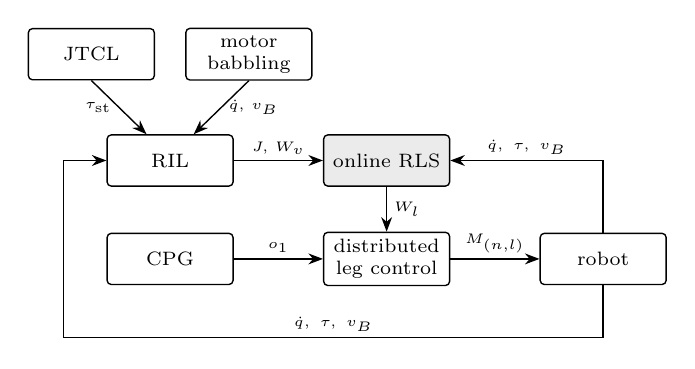
\begin{tikzpicture}[
      font=\scriptsize,
      box/.style={draw, rounded corners=1.5pt, align=center,
                  inner sep=2.5pt, minimum height=6.5mm, minimum width=16mm},
      >=Stealth, line width=0.5pt
    ]
    % --- initialization sources -------------------------------------------
    \node[box] (jtcl) at (-1.0,2.6)  {JTCL};
    \node[box] (bab)  at ( 1.0,2.6)  {motor\\babbling};

    % --- main blocks -------------------------------------------------------
    \node[box] (ril) at (0,1.25)   {RIL};
    \node[box, fill=black!8] (rls) at (2.75,1.25) {online RLS};
    \node[box] (cpg) at (0,0)      {CPG};
    \node[box] (ctl) at (2.75,0)   {distributed\\leg control};
    \node[box] (rob) at (5.5,0)    {robot};

    % --- initialization data into RIL --------------------------------------
    \draw[->] (jtcl.south) -- node[left=-0.3mm, font=\tiny] {$\tau_\mathrm{st}$}
              ([xshift=-3mm]ril.north);
    \draw[->] (bab.south)  -- node[right=-0.3mm, font=\tiny] {$\dot q,\,\vB$}
              ([xshift=3mm]ril.north);

    % --- forward path ------------------------------------------------------
    \draw[->] (ril) -- node[above=-0.5mm, font=\tiny] {$\Jm,\,W_v$} (rls);
    \draw[->] (cpg) -- node[above=-0.5mm, font=\tiny] {$o_1$} (ctl);
    \draw[->] (ctl) -- node[above=-0.5mm, font=\tiny] {$M_{(n,l)}$} (rob);
    \draw[->] (rls.south) -- node[right=-0.3mm, font=\tiny] {$W_l$} (ctl.north);

    % --- feedback to RIL (offline identification data) ---------------------
    \coordinate (fb) at (-1.35,-1.0);
    \draw (rob.south) |- node[above=-0.5mm, pos=0.75, font=\tiny]
          {$\dot q,\ \tau,\ \vB$} (fb);
    \draw[->] (fb) |- (ril.west);

    % --- feedback to online RLS -------------------------------------------
    \coordinate (fbr) at (5.5,1.25);
    \draw (rob.north) -- (fbr);
    \draw[->] (fbr) -- node[above=-0.5mm, font=\tiny] {$\dot q,\ \tau,\ \vB$} (rls.east);
  \end{tikzpicture}
  \caption{Overview of the Online RLS in RIL architecture. During initialization, RIL obtains
  the vertical weights $W_v$ from standing joint torques collected under JTCL, and
  estimates the joint-to-body linear-velocity map $J$ from motor-babbling data using
  batch LS. Online RLS in RIL initializes the recursion with this estimate and updates the
  horizontal part of $J$ during locomotion. At each control cycle, the updated
  controller weights $W_l$ and the CPG output generate the joint position commands.}
  \label{fig:arch}
\end{figure}

\section{METHODOLOGY}
\label{sec:method}

% \oldtext{Fig.~\ref{fig:arch} shows the architecture. Consider a robot with $L$
% legs of $n$ joints each. Lowercase symbols denote single-sample row vectors and
% uppercase symbols denote matrices of stacked samples. For leg $l$ at sample $t$
% we write $\vj(t)=[\dot q_1(t),\dots,\dot q_n(t)]\in\mathbb{R}^{1\times n}$ for
% the joint velocities and $\vB(t)=[v_x(t),v_y(t),v_z(t)]\in\mathbb{R}^{1\times
% 3}$ for the body velocity, and stack $T$ samples into
% $V_j\in\mathbb{R}^{T\times n}$ and $V_B\in\mathbb{R}^{T\times 3}$.}

\newtext{Fig.~\ref{fig:arch} provides an overview of the proposed approach.
RIL consists of Joint-torque Contribution Learning (JTCL) for vertical weight learning
and motor babbling for horizontal weight learning. The procedure starts with a brief
identification phase while the robot remains standing. Joint-torque contribution learning (JTCL)
uses joint-torque feedback to obtain the vertical controller weights $W_v$, while motor babbling
provides motion data from which batch LS estimates the joint-to-body velocity map
$J$. The horizontal controller weights $W_h$ are derived from this map and
combined with $W_v$ into the per-leg controller weights $W_l$ that translate the
CPG rhythm into joint position commands. After locomotion starts, RIL incorporates
an online RLS step. Starting from the batch LS estimate, it leverages the same motion feedback
to further adjust the horizontal controller weights during walking. The next subsections present
the mathematical formulation of each stage.}

\subsection{Rapid Innate Learning}
\label{sec:ril}

% \oldtext{RIL is prior work \cite{leung2023,ril} and none of it is claimed here.
% We state it in full rather than in summary, because \cite{ril} is not yet
% available to the reader and because Section~\ref{sec:online} modifies one
% specific step of it. RIL produces one weight matrix per leg,}
% {\color{red}
% \begin{equation*}
%   \begin{aligned}
%     W_l &= \begin{bmatrix} W_{h_{[n\times2]}} & W_{v_{[n\times1]}} \end{bmatrix}
%         \in \mathbb{R}^{n\times 3}\\[2pt]
%         &= \begin{pmatrix}
%              w_{1,x} & w_{1,y} & w_{1,z}\\
%              \vdots  & \vdots  & \vdots \\
%              w_{n,x} & w_{n,y} & w_{n,z}
%            \end{pmatrix},
%   \end{aligned}
% \end{equation*}}
% \oldtext{in which each row corresponds to one joint and each column to the
% contribution of that joint to body velocity along the $x$-, $y$- and $z$-axes.
% The horizontal part $W_h$ drives the return and power strokes and the vertical
% part $W_v$ drives lift-off and touch-down.}

\newtext{RIL is a method introduced in \cite{leung2023,ril}. Here, we present a brief overview and summary of this learning framework. For each leg $l$ with $n$ actuated joints, RIL constructs a controller weight matrix $W_l$ as}
{\color{black}
\begin{equation}
  \begin{aligned}
    W_l &= \begin{bmatrix} W_{h_{[n\times2]}} & W_{v_{[n\times1]}} \end{bmatrix}
        \in \mathbb{R}^{n\times 3}\\[2pt]
        &= \begin{pmatrix}
             w_{1,x} & w_{1,y} & w_{1,z}\\
             \vdots  & \vdots  & \vdots \\
             w_{n,x} & w_{n,y} & w_{n,z}
           \end{pmatrix},
  \end{aligned}
  \label{eq:wl}
\end{equation}}
\newtext{Each row of $W_l$ corresponds to one joint, while its columns describe
that joint's contribution to body linear velocity along the $x$-, $y$-, and
$z$-axes. The horizontal weights $W_h$ govern the power and return strokes,
whereas the vertical weights $W_v$ govern lift-off and touch-down.}

\subsubsection{Joint-torque contribution learning (JTCL)}
% \oldtext{While the robot stands, each leg carries a share of the ground reaction
% force, and each joint must generate torque to counteract it. The vertical weights
% are the normalized torque contributions,}
\newtext{While the robot is standing, ground-reaction forces load each leg, and
its joints generate torques to support the body. JTCL defines each joint's
vertical weight as its signed torque normalized by the sum of the torque
magnitudes within that leg,}
% {\color{red}
% \begin{equation}
%   W_{v_{[n\times1]}} \leftarrow w_{n,z}
%     = \frac{\tau_n}{\sum_{n=1}^{N}|\tau_n|},
% \end{equation}
% }
{\color{black}
\begin{equation}
  W_{v_{[n\times1]}} \leftarrow w_{n,z}
    = \frac{\tau_n}{\sum_{i=1}^{N}|\tau_i|},
    \qquad n=1,\ldots,N,
  \label{eq:jtcl}
\end{equation}
}
% \oldtext{where $\tau_n$ is the torque feedback of joint $n$ and $N$ the number of
% joints in the leg. The magnitude gives the joint's share of body weight and the
% sign gives the direction of the torque produced by the ground reaction force.}
\newtext{where $\tau_n$ is the torque measured at joint $n$, and $N$ is the
number of actuated joints in the leg. This normalization represents each joint's
signed relative torque contribution; it is not a direct estimate of joint power,
ground-reaction force, or supported body weight.}
% \oldtext{Equation~(\ref{eq:jtcl}) is evaluated once per control cycle over an
% initial standing interval of $N_0$ cycles, with the torques accumulated rather
% than sampled instantaneously, since on hardware the instantaneous estimate is too
% noisy to give a usable ratio. $W_v$ is then held fixed for the rest of the run:
% we refine only $W_h$, and leave recursive refinement of $W_v$ to future work.}
\newtext{During an initial standing phase, the robot is held stationary to allow the joint-torque feedback to converge. At the end of this settling period, the converged torque readings are sampled and substituted
into Eq.~(\ref{eq:jtcl}) to compute $W_v$. Waiting for convergence avoids using
transient torque measurements and provides a more robust estimate. The resulting
$W_v$ remains fixed during locomotion.}

\subsubsection{Motor babbling}
% \oldtext{Babbling excites the robot's joints and records how the body responds
% \cite{leung2023,ril}. One leg is designated active and the other legs are left
% uncommanded. The active leg's joints are babbled in sequence, $j_1$ then $j_2$
% then $j_3$, and each joint is treated as follows. For $N_b$ control cycles the
% joint receives a piecewise-constant position reference, redrawn every $N_r$
% cycles from a uniform distribution $\mathcal{U}(-a,a)$. The joint is then
% returned to its neutral angle and held for $N_s$ cycles before the next joint
% begins. Throughout the babbling cycles, and for every leg rather than only the
% active one, the $n$ joint velocities and the corresponding body velocity are
% appended to the record. The settling cycles are excluded, so each leg contributes
% $T = n N_b$ samples. We use $N_b=200$, $N_r=35$, $N_s=50$ and $a=0.2$\,rad,
% which with $n=3$ gives $T=600$ samples per leg and $750$ cycles of babbling.}
\newtext{After JTCL, motor babbling excites the joints while recording the
resulting body motion \cite{leung2023,ril}. One leg is designated as active,
while the remaining legs are left uncommanded. The three joints of the active leg
are excited sequentially. Each joint receives a piecewise-constant position
reference for $200$ control cycles. A new reference is drawn every $35$ cycles
from a uniform distribution over $[-0.2,0.2]$\,rad. The joint is then returned
to its neutral angle and allowed to settle for $50$ cycles before excitation
proceeds to the next joint. During each excitation cycle, the joint velocities of
every leg and the synchronized body linear velocity are recorded. Excluding the
settling intervals gives $T=600$ retained samples per leg from a $750$-cycle
sequence.}

% \oldtext{Sampling every leg while commanding only one makes the procedure cheap.
% The active leg's motion is transmitted through the body and the ground contacts
% to the passive legs, whose compliant joints deflect measurably. Those deflections
% are not commanded, but they are observed and paired with the same body velocity,
% so one babbling sequence yields a separate regression problem per leg and the
% babbling cost does not grow with the number of legs \cite{ril}.}

\newtext{Although only one leg is commanded, the resulting motion is transmitted
through the body and ground contacts, producing measurable deflections in the
compliant joints of the passive legs. Pairing the velocity of each leg with the
same synchronized body linear velocity yields a separate regression dataset for
every leg. Consequently, one motor-babbling sequence identifies all per-leg maps,
and the identification duration does not increase with the number of legs
\cite{ril}.}

% \oldtext{The relationship between joint and body velocity is modeled as a linear
% transformation with Jacobian matrix $\Jm\in\mathbb{R}^{n\times3}$,}
\newtext{For leg $l$ at control sample $t$, let
$v_{j,l}(t)=[\dot q_{1,l}(t),\ldots,\dot q_{N,l}(t)]\in
\mathbb{R}^{1\times N}$ denote the measured joint-velocity row vector, and let
$\vB(t)=[v_x(t),v_y(t),v_z(t)]\in\mathbb{R}^{1\times3}$ denote the measured body
linear-velocity row vector. Stacking $T$ synchronized samples gives
$V_{j,l}\in\mathbb{R}^{T\times N}$ and $V_B\in\mathbb{R}^{T\times3}$, where
$V_B$ is common to all legs. The regression is performed independently for each
leg. Motor babbling approximates the local input--output relationship between
joint velocity and body linear velocity using the regression-coefficient matrix
$\Jm\in\mathbb{R}^{N\times3}$,}
\begin{equation}
  \begin{aligned}
    \vB(t) &= v_{j,l}(t)\,\Jm, \qquad V_B = V_{j,l}\,\Jm ,\\[2pt]
    \Jm &= \begin{pmatrix}
             J_{1x} & J_{1y} & J_{1z}\\
             \vdots & \vdots & \vdots\\
             J_{Nx} & J_{Ny} & J_{Nz}
           \end{pmatrix} ,
  \end{aligned}
  \label{eq:babble}
\end{equation}
% \oldtext{so that row $n$ of $\Jm$ holds the contribution of joint $n$ to the
% three body-velocity components. The system is overdetermined, and $\Jm$ is
% estimated in the least-squares sense by the normal equations,}
\newtext{Each row $n$ of $\Jm$ represents the contribution of joint $n$ to the
three components of body linear velocity. Because the number of recorded samples
is greater than the number of joints, the batch LS estimate is obtained from the
normal equations,}
\begin{equation}
  \Jm = \bigl(V_j^{\top}V_j\bigr)^{-1}V_j^{\top}V_B ,
  \label{eq:batchls}
\end{equation}
% \oldtext{solved once per leg when babbling ends.}
\newtext{Equation~(\ref{eq:batchls}) is the closed-form normal-equation solution
to a batch multi-output ordinary least-squares (OLS) regression. Specifically,
it estimates $J$ by minimizing the total squared prediction error
$\lVert V_B-V_jJ\rVert_F^2$ over the $T$ motor-babbling samples. The resulting
matrix maps measured joint velocities to the least-squares prediction of the
three body linear-velocity components. This solution is unique when $V_j$ has
full column rank, in which case $V_j^{\top}V_j$ is nonsingular. In the
implementation, we use Gauss--Jordan elimination to solve the equivalent normal
equations $(V_j^{\top}V_j)J=V_j^{\top}V_B$, rather than explicitly forming the
matrix inverse. The regression is solved independently for each leg after
babbling. Thus, $J$ is a data-driven local linear map expressed in the row-vector
convention of Eq.~(\ref{eq:babble}), rather than an analytically derived
geometric Jacobian.}
% \oldtext{Horizontal locomotion uses only the $x$ and $y$ columns,}
\newtext{Only the $x$- and $y$-axis columns of $J$ are used to construct the
horizontal weights $W_h$; the vertical weights $W_v$ are obtained separately by
JTCL,}
\begin{equation}
  \Jm_{xy} = \Jm_{(:,1:2)}\in\mathbb{R}^{N\times2},
  \qquad
  W_h = \mathrm{norm}(-\Jm_{xy}),
  \label{eq:wh}
\end{equation}
% \oldtext{where the operator normalizes each column by the sum of absolute values
% in that column,}
\newtext{where $\mathrm{norm}$ independently normalizes each column by
its sum of absolute values,}
\begin{equation}
  \bigl[\mathrm{norm}(-\Jm_{xy})\bigr]_{n,k}
    = \frac{-(\Jm_{xy})_{n,k}}{\sum_{r=1}^{N}\bigl|(\Jm_{xy})_{r,k}\bigr|} ,
  \label{eq:norm}
\end{equation}
% \oldtext{with $i$ the row index of the joint being normalized and
% $k\in\{1,2\}$ the $x$- or $y$-axis column. The negative sign converts the map
% from joint velocity to body velocity into controller weights that multiply the
% CPG signal directly.}
\newtext{Here, $n\in\{1,\ldots,N\}$ indexes the joint and $k\in\{1,2\}$
indexes the horizontal axis. The leading negative sign converts the identified
joint-to-body velocity map to the sign convention used by the CPG controller.}

% \oldtext{The complete sequence is therefore $N_0$ standing cycles, $750$
% babbling cycles and one batch solve. At a $0.02$\,s control period the robot
% begins walking about $17$\,s after start-up. Equation~(\ref{eq:batchls}) is the
% step this paper replaces.}
\newtext{RIL initialization proceeds in three stages: the standing JTCL phase,
a $750$-cycle motor-babbling sequence, and one batch LS estimate of $J$ for each
leg. At the $0.02$\,s simulation time step, the motor-babbling stage lasts
$15$\,s. The estimated joint-to-body velocity maps are converted into controller
weights used to generate joint commands. In RIL, these maps remain fixed during
locomotion. In Online RLS in RIL, each per-leg batch estimate from
Eq.~(\ref{eq:batchls}) initializes the recursion, which continues to
update the corresponding map while the robot walks.}

\subsection{Distributed Leg Control}
\label{sec:dlc}

Rhythm is generated by a two-neuron SO(2) oscillator
\cite{pasemann2003,miguelblanco2020},
\begin{equation}
  \begin{pmatrix} o_1(t) \\ o_2(t) \end{pmatrix}
  \leftarrow \tanh
  \begin{pmatrix} w^c_{11}o_1(t-1) + w^c_{12}o_2(t-1) \\
                  w^c_{21}o_1(t-1) + w^c_{22}o_2(t-1) \end{pmatrix},
  \label{eq:cpg}
\end{equation}
with self-connections $w^c_{11}=w^c_{22}=1.4$ and mutual connections
$w^c_{12}=0.23$ and $w^c_{21}=-0.23$. These weights place the network in a
quasi-periodic regime \cite{pasemann2003} and give a stepping frequency of
approximately $0.76$\,Hz. Motor commands follow in matrix form as
\begin{equation}
  M_{(n,l)}(t) = p_l\,o_1(t)\,(W_l)_{n,:}\cdot K + b_n ,
  \label{eq:motor}
\end{equation}
where $M_{(n,l)}(t)$ is the command to joint $n$ of leg $l$, $b_n$ is the joint
bias and $p_l\in\{+1,-1\}$ is the predefined phase relation between legs, set to
$+1$ for R1 and L2 and $-1$ for R2 and L1, where R1 and R2 denote the right
front and right hind legs and L1 and L2 the left front and left hind legs.
Multiplying $o_1(t)$ by $-1$ shifts
the phase of those legs by $180^\circ$, which produces the alternating diagonal
pattern of a trot. The gain vector selects swing or stance according to the sign
of $o_1(t)p_l$,
\begin{equation}
  K = \begin{cases}
    K_{sw} = [k_x, k_y, k_z]^\top
      & \text{if } o_1(t) p_l > 0 \\
    K_{st} = [k_x, k_y, 0]^\top
      & \text{if } o_1(t) p_l < 0
  \end{cases},
  \label{eq:gain}
\end{equation}
so that setting $k_z=0$ during stance removes the vertical oscillation and holds
the leg at its neutral height. The gains $k_x$ and $k_y$ set the commanded
direction of travel, $k_z$ sets the vertical oscillation, and these are the only
quantities set by hand.

\subsection{Online Recursive Least-Squares Adaptation}
\label{sec:online}

% \oldtext{The mechanism described up to this point is inherited. The proposed
% refinement alters a single step of it: the batch solve of
% (\ref{eq:batchls}) is no longer the final estimate. The gait, the oscillator, and
% the babbling schedule are unchanged from the baseline. Because
% (\ref{eq:batchls}) is identified during babbling, and walking differs from
% babbling as set out in Section~\ref{sec:intro}, we treat the batch solution as an
% initial condition and continue to estimate $\Jm$ during walking from the same
% joint-velocity and body-velocity signals that (\ref{eq:babble}) uses.}

\newtext{Online RLS in RIL retains the JTCL procedure, motor-babbling schedule, CPG, and
distributed joint controller of RIL. The difference is what happens after the
batch LS identification in Eq.~(\ref{eq:batchls}). RIL keeps each map $J_l$
fixed, whereas Online RLS in RIL uses the batch estimate as the starting point of an
online RLS estimator. During walking, the estimator updates each leg's map once
per control cycle using the joint-velocity and synchronized body-linear-velocity
measurements defined in Eq.~(\ref{eq:babble}).}

% \oldtext{For each leg we maintain an estimate $\hat{\Jm}_l$ and a covariance
% $P_l\in\mathbb{R}^{N\times N}$, initialized from the batch result,}
\newtext{For each leg $l$, the estimator stores the current map
$\hat{\Jm}_l\in\mathbb{R}^{N\times3}$ and the RLS covariance matrix
$P_l\in\mathbb{R}^{N\times N}$. The map relates the leg's $N$ joint velocities
to the three components of body linear velocity. The covariance represents the
estimator's uncertainty and determines how strongly new measurements can change
the map. These quantities are initialized as}
\begin{equation}
  \hat{\Jm}_l(0) = \Jm_l, \qquad P_l(0) = p_0 I_N ,
  \label{eq:seed}
\end{equation}
\newtext{In Eq.~(\ref{eq:seed}), the index $0$ denotes the start of locomotion,
before the first online update, and $\Jm_l$ is the batch LS map learned for leg
$l$ during motor babbling. We set $p_0=10$. Because the simulated robot has
$N=3$ joints per leg, $I_N=I_3$ is a $3\times3$ identity matrix, with ones on
its diagonal and zeros elsewhere. Thus, $P_l(0)=10I_3$ assigns the same initial
uncertainty to all three joint directions and assumes no initial
cross-correlation between them.}

\newtext{The batch seed is needed to avoid a cold start. Initializing
$\hat{\Jm}_l(0)=0$ would provide no valid morphology-dependent horizontal map
for generating the walking motion needed for online identification. Although
the batch estimate may be biased because it is identified while the robot is
standing, it provides a functional initial controller that RLS can subsequently
refine using locomotion data.}
% \oldtext{and update them once per control cycle by exponentially weighted
% recursive least squares \cite{ljung1999,astrom1995},}
\newtext{Once walking begins, the robot reads $v_{j,l}(t)$ and $\vB(t)$ at each
control cycle and applies the following exponentially weighted RLS updates
\cite{ljung1999,astrom1995}:}
\begin{align}
  k_l(t) &= \frac{P_l(t-1)\,
                 v_{j,l}(t)^{\top}}
                 {\lambda +
                 v_{j,l}(t)\,P_l(t-1)\,
                 v_{j,l}(t)^{\top}},
  \label{eq:rlsk}\\
  \hat{\Jm}_l(t) &= \hat{\Jm}_l(t-1)
       + k_l(t)\bigl[\vB(t) -
       v_{j,l}(t)\,\hat{\Jm}_l(t-1)\bigr],
  \label{eq:rlstheta}\\
  P_l(t) &= \lambda^{-1}\bigl[P_l(t-1) - k_l(t)\,
       v_{j,l}(t)\,P_l(t-1)\bigr].
  \label{eq:rlsp}
\end{align}
% \oldtext{The bracketed term in (\ref{eq:rlstheta}) is the prediction error, the
% difference between the measured body velocity and the value the current estimate
% predicts from the measured joint velocities. The forgetting factor
% $\lambda=0.995$ discounts older samples, so the estimate follows the walking
% conditions rather than the babbling data that produced the seed. After each
% update, $W_h$ is recomputed from $\hat{\Jm}_l$ by (\ref{eq:wh}) and
% (\ref{eq:norm}) and reassembled with $W_v$ into $W_l$ by (\ref{eq:wl}). The
% gait in (\ref{eq:motor}) then uses the refined map in the same cycle.}
\newtext{The three equations are applied in sequence. First,
Eq.~(\ref{eq:rlsk}) computes the gain
$k_l(t)\in\mathbb{R}^{N\times1}$, which controls how strongly the current
measurement changes the map. Greater uncertainty in the direction of the
current joint motion produces a larger gain. Second, the bracketed term in
Eq.~(\ref{eq:rlstheta}) computes the prediction error, defined as the measured
body linear velocity minus the velocity predicted by the previous map. The gain
scales this error before it is added to $\hat{\Jm}_l(t-1)$. Third,
Eq.~(\ref{eq:rlsp}) updates $P_l(t)$ for the next control cycle. Informative
joint motion reduces uncertainty along the observed direction, which decreases
future gains in directions that are already well identified.}

\newtext{The forgetting factor $\lambda=0.995$ reduces the influence of older samples,
allowing the map to track the conditions encountered during walking. At the
$0.02$\,s simulation control period, the nominal effective memory
$1/(1-\lambda)=200$ samples corresponds to approximately $4$\,s.}

\newtext{After the RLS update, the refined map is converted into $W_h$ using
Eqs.~(\ref{eq:wh}) and (\ref{eq:norm}). The horizontal weights are then combined
with the fixed $W_v$ to form $W_l$ using Eq.~(\ref{eq:wl}), and
Eq.~(\ref{eq:motor}) uses the updated weights to generate the next joint
command.}

% \oldtext{The seed determines convergence. Starting from
% $\hat{\Jm}_l(0)=0$, the robot cannot yet walk, so the estimator receives no
% informative excitation. Starting from the babbling solution, the estimate is
% biased but usable, and the robot walks while the estimate improves. We use
% $p_0=10$.}

\subsection{Joint-Motion Gating and Covariance Bounding}
\label{sec:stop}

% \oldtext{With $\lambda<1$, $P_l$ grows whenever incoming data carry no
% information, and an inflated $P_l$ turns the next informative sample into a large
% parameter jump. A walking robot produces exactly this pattern, because a leg in
% stance is loaded but barely moving. Two rules bound the effect.}
\newtext{During locomotion, a leg may remain nearly stationary during part of
the gait cycle, giving $v_{j,l}(t)\approx0$. Such a sample contains little
information about the relationship between joint velocity and body velocity. In
this case, the gain in Eq.~(\ref{eq:rlsk}) approaches zero, so the map estimate
changes very little. However, the covariance update in
Eq.~(\ref{eq:rlsp}) approaches
$P_l(t)=\lambda^{-1}P_l(t-1)$. Because $\lambda<1$, repeated low-motion samples
can gradually increase $P_l$. When informative joint motion resumes, the
inflated covariance may produce a large gain and an abrupt change in the map.
Online RLS in RIL therefore applies two update rules: joint-motion gating and covariance bounding.}

\newtext{ Before applying the RLS equations, the
algorithm checks the magnitude of the current joint-velocity vector. If
$\lVert v_{j,l}(t)\rVert<\varepsilon$, where $\varepsilon=10^{-4}$, the sample
is considered insufficiently informative and the update is skipped. Both
$\hat{\Jm}_l$ and $P_l$ retain their previous values. This prevents low-motion
samples from increasing the covariance without improving the map estimate.}

\newtext{After an accepted RLS update, the
algorithm checks the covariance trace, which summarizes the total uncertainty
across the estimated parameters. If
$\operatorname{tr}\!\left(P_l(t)\right)>P_{\max}$, with $P_{\max}=150$, the
covariance is rescaled as
$P_l(t)\leftarrow P_{\max}P_l(t)/\operatorname{tr}\!\left(P_l(t)\right)$.
This operation limits the magnitude of future RLS gains while preserving the
relative uncertainty among the joint directions.}

%%%%%%%%%%%%%%%%%%%%%%%%%%%%%%%%%%%%%%%%%%%%%%%%%%%%%%%%%%%%%%%%%%%%%%%%%%%%%%%%
\section{SIMULATION EXPERIMENTS}
\label{sec:sim}

\subsection{Robot Simulation Setup}

\newtext{The simulated robot is a four-legged platform with three joints per
leg, as shown in Fig.~\ref{fig:restime}. The robot is modeled in CoppeliaSim
\cite{rohmer2013}, and each joint uses compliant spring--damper control with
$k=8.0$ and $c=0.2$. Body linear velocity is measured using markers attached to
the robot body.}

We compare the following two controllers:

\begin{itemize}
    \item \emph{Baseline RIL}: the controller described in Section~\ref{sec:ril}. For each leg, the velocity map $\Jm_l$ is estimated once using the batch LS solution in Eq.~(\ref{eq:batchls}) and remains fixed throughout locomotion.
    \item \emph{Online RLS in RIL}: the proposed controller. It is initialized using the same batch LS procedure, but after walking begins, the velocity map is continuously refined using the recursive updates in Eqs.~(\ref{eq:rlsk})--(\ref{eq:rlsp}).
\end{itemize}

All other experimental settings are identical between the two controllers, including the simulation scene, oscillator parameters, motor-babbling schedule, and commanded gains $k_x=0.6$, $k_y=0$, and $k_z=1.0$, corresponding to forward locomotion.

Each run lasts $27$\,s and consists of two phases:
\begin{itemize}
    \item the first $17$\,s comprise joint-torque contribution learning, motor babbling, and computation of the initial batch LS estimate; and
    \item the final $10$\,s comprise the walking phase.
\end{itemize}

During walking, Online RLS in RIL recursively updates the velocity map using RLS, whereas baseline RIL retains the initial batch estimate without further adaptation.
Both controllers estimate $\Jm$ from independently generated babbling data. All other controller and scene settings are identical, although the random trials are not paired between conditions.
We perform $100$ runs for each controller and compute all metrics over the walking phase.
Runs that travel less than $1$\,m are classified as gait failures and are retained in the reported statistics.
The evaluation metrics are defined as follows:
\begin{itemize}
    \item \emph{Heading error}: the angle between the commanded walking direction and the net displacement vector measured from gait onset.
    \item \emph{Lateral drift}: the component of the net displacement perpendicular to the commanded walking direction.
    \item \emph{Straightness}: the ratio of net displacement to total path length. A value of one indicates a perfectly straight trajectory.
    \item \emph{Mean speed}: the average speed of the robot during the walking phase.
\end{itemize}

\subsection{Results}

% \oldtext{Fig.~\ref{fig:simpaths} shows every run. The baseline walks a comparable
% distance in most trials, but travels in a different direction each time, with
% final headings spanning $-4.4^\circ$ to $+102.7^\circ$; five runs stalled before
% the end of the walking phase. The online runs all sustained the gait, with final
% headings spanning $-16.3^\circ$ to $+16.2^\circ$.}
\newtext{Fig.~\ref{fig:simpaths} shows the trajectory of every run. RIL travels a
comparable distance in most trials, but the final trajectory heading varies
substantially across runs, spanning $-4.4^\circ$ to $+102.7^\circ$. Five RIL
runs traveled less than $1$\,m and were classified as gait failures. All Online RLS in RIL runs sustained the gait, with final trajectory headings confined to
$-16.3^\circ$ to $+16.2^\circ$.}

\begin{figure}[t]
  \centering
  \includegraphics[width=\columnwidth]{fig_sim_paths.pdf}
  % \caption{\oldtext{Body-centre trajectories during the walking phase, all runs
  % superimposed and re-referenced to gait onset (cross). Dots mark run ends. (a)
  % One-shot batch estimation, $100$ runs. (b) Proposed online recursive
  % refinement, $100$ runs. In each panel the median run, whose endpoint best
  % represents the group, is drawn in full opacity and the remaining runs in
  % reduced opacity. The protocol is identical, and only the online update
  % differs.}}
  \caption{\newtext{Body-center trajectories during the walking phase, expressed
  relative to the position at gait onset (cross). Dots mark final positions. (a)
  RIL with one-shot batch LS, $100$ runs. (b) Online RLS in RIL, $100$ runs. For
  visibility, one run is drawn in full opacity and the remaining runs in reduced
  opacity. Controller settings are identical, but independently generated
  babbling trials are used for the two conditions.}}
  \label{fig:simpaths}
\end{figure}

\begin{figure}[t]
  \centering
  \includegraphics[width=\columnwidth]{fig_results_time.pdf}
  \caption{Behavior over time during walking. (a),(b) CoppeliaSim
  captures of one representative run per controller, successive poses
  superimposed, rescaled and aligned on the horizon so the floor tiles give a
  common scale. (c) Normalized horizontal weight matrix $W_h$ of leg R1 at four
  instants, showing the map being revised as the robot walks. (d) Straightness
  and (e) absolute heading error against time since gait onset. Lines are means
  across runs, and bands span the observed range.}
  \label{fig:restime}
\end{figure}

\begin{figure}[t]
  \centering
  \includegraphics[width=\columnwidth]{fig_boxplot.pdf}
  \caption{\newtext{Distributions of heading error, lateral drift, straightness,
  and mean speed for RIL ($n=100$) and Online RLS in RIL ($n=100$). Individual trials
  are overlaid as points.}}
  \label{fig:box}
\end{figure}
% \oldtext{Fig.~\ref{fig:restime} shows the difference over time. Panels~(a) and
% (b) show the two controllers in the simulator, with the successive poses of one
% representative run superimposed. Under batch estimation the robot drifts away
% from the commanded direction and its yaw changes as it goes, so the robot
% advances diagonally across the floor. Under online refinement they advance along
% a nearly straight line at almost constant depth. Panel~(c) shows the weight
% matrix of one leg being revised during locomotion rather than staying at its
% babbling value. Panel~(d) shows straightness settling near $0.58$ for the online
% controller against roughly $0.47$ for the baseline. Panel~(e) shows the largest
% difference: baseline heading error grows steadily through the run, reaching a
% mean of about $26^\circ$ rather than settling to a constant offset, whereas the
% online controller keeps its mean heading error near $6^\circ$ throughout.}
\newtext{Fig.~\ref{fig:restime} compares the two controllers over time.
Panels~(a) and (b) show superimposed poses from representative RIL and Online RLS in RIL
runs, respectively. With RIL, the trajectory progressively deviates from the
commanded direction. With Online RLS in RIL, the robot follows a nearly straight
trajectory. Panel~(c) shows the horizontal weight matrix of one leg changing
during locomotion as the underlying velocity-map estimate is updated.
Panel~(d) shows straightness approximately $0.58$ for Online RLS in RIL,
compared with approximately $0.47$ for RIL. Panel~(e) shows the largest
difference: the mean absolute heading error of RIL increases throughout the
walking phase and reaches approximately $26^\circ$, whereas Online RLS in RIL maintains
a mean absolute heading error near $6^\circ$.}

% \oldtext{Fig.~\ref{fig:box} summarizes the end-of-run distributions. Mean
% absolute heading error falls from $26.3^\circ$ to $5.5^\circ$ and mean absolute
% lateral drift from $1.02$\,m to $0.25$\,m. Forward speed is unchanged, $0.263$
% against $0.253$\,m/s, and net displacement is comparable, $2.63$ against
% $2.53$\,m. The online update therefore does not increase speed. It aligns the
% traveled distance with the commanded direction and reduces the variation between
% runs, with the standard deviation of net displacement falling from $0.61$\,m to
% $0.14$\,m.}
\newtext{Fig.~\ref{fig:box} summarizes the distributions of heading error,
lateral drift, straightness, and mean speed. From RIL to Online RLS in RIL, mean
absolute heading error decreases from $26.3^\circ$ to $5.5^\circ$, mean absolute
lateral drift decreases from $1.02$\,m to $0.25$\,m, and mean forward speed
remains comparable at $0.263$ and $0.253$\,m/s, respectively
(Fig.~\ref{fig:box}). These results indicate that the principal observed effect
is improved directional consistency rather than increased speed. Additional
trajectory summaries, which are not plotted in Fig.~\ref{fig:box}, show
comparable mean net displacement ($2.63$ and $2.53$\,m) and a reduction in its
standard deviation from $0.61$\,m to $0.14$\,m for RIL and Online RLS in RIL,
respectively.}

% \oldtext{Fig.~\ref{fig:stop} supports the stop-learning mechanism of
% Section~\ref{sec:stop}. Each leg's estimate departs from its seed and then holds a
% bounded offset for the rest of the run: continued adaptation without the
% covariance wind-up that intermittent stance excitation would otherwise cause.}
\newtext{Fig.~\ref{fig:stop} shows the estimator behavior when both update rules from Section~\ref{sec:stop},
joint-motion gating and covariance bounding, are enabled. The plotted quantity is the
Frobenius-norm distance between each leg's current velocity-map estimate and its
batch seed. The estimates move away from their seeds but remain bounded over the
reported walking interval. This result is consistent with bounded estimator
updates, although it does not isolate the contribution of either joint-motion gating or covariance bounding.}

\begin{figure}[t]
  \centering
  \includegraphics[width=\columnwidth]{fig_stoplearn.pdf}
  \caption{Distance of each leg's estimate from its seed during
  walking. The estimates settle at bounded offsets rather than drifting,
  indicating that the stop-learning mechanism holds the recursion stable under
  intermittent excitation.}
  \label{fig:stop}
\end{figure}

%%%%%%%%%%%%%%%%%%%%%%%%%%%%%%%%%%%%%%%%%%%%%%%%%%%%%%%%%%%%%%%%%%%%%%%%%%%%%%%%
\section{SIM-TO-REAL FEASIBILITY STUDY}
\label{sec:sim2real}

This section is a feasibility study of the inherited batch mechanism on
a Unitree Go2 quadruped, separate from the contribution evaluated in
Section~\ref{sec:sim}. The controller deployed here is exactly
Sections~\ref{sec:ril} and \ref{sec:dlc} with the batch solve of
(\ref{eq:batchls}). \emph{The recursive estimator of Section~\ref{sec:online} was
not run on hardware}, and no result in this section supports a claim about online
refinement. The purpose is to establish that the identification procedure
executes on a physical platform at all, and to identify the constraints a future
online deployment must satisfy. Only the procedure crosses over,
(\ref{eq:jtcl})--(\ref{eq:batchls}), not a fitted quantity: the matrices used on
the Go2 were never computed in simulation, so there is no sim-to-real parameter
mismatch to bridge, and no domain randomization or fine-tuning stage is required.



\subsection{Hardware Setup}

The controller runs as a single $500$\,Hz process publishing joint position
commands ($K_p=60$, $K_d=5$) over the robot's low-level interface, with the
manufacturer's motion service released so that it does not compete with those
commands. Joint velocities and estimated torques arrive on the same interface.
Body velocity, required by
(\ref{eq:babble}), is supplied by a contact-aided
invariant extended Kalman filter \cite{hartley2020} running as a separate node, a
standard choice for legged state estimation \cite{yang2023}.

We record three integration problems, none of which appears in
simulation. First, the batch solve for four legs blocks long enough to miss
control cycles, and a missed cycle trips a watchdog that makes the robot lose its
balance and fall over.
A parallel thread holds the standing posture at $500$\,Hz for the duration
of the solve. Second, the transition from the manufacturer's posture to the
learned gait must be interpolated over roughly a second, or the robot lurches at
handover. Third, the torque estimate of (\ref{eq:jtcl}) is unusable
instantaneously and requires the accumulation over $N_0=500$ cycles noted in
Section~\ref{sec:ril}.

\subsection{Results}

Three commanded conditions---forward,
backward, and in-place---were obtained by changing only $k_x$, with telemetry
logged at $1$\,Hz (Fig.~\ref{fig:go2snap}).

\begin{table}[t]
  \caption{Locomotion measured on the Unitree Go2}
  \label{tab:real}
  \centering
  \setlength{\tabcolsep}{2.5pt}
  \footnotesize
  \begin{tabular}{lcccc}
    \toprule
    \shortstack{Commanded\\direction} &
    \shortstack{Number\\of runs} &
    \shortstack{Run duration\\{[s]}} &
    \shortstack{Distance traveled\\{[m]}} &
    \shortstack{Travel direction\\{[deg]}} \\
    \midrule
    Forward   & 6 & $123 \pm 26$ & $0.74 \pm 0.26$ & $-19.6 \pm 13.1$ \\
    Backward  & 5 & $ 81 \pm  2$ & $0.41 \pm 0.05$ & $-158.2 \pm 4.8$ \\
    In-place  & 2 & $ 76 \pm 16$ & $0.07 \pm 0.05$ & --- \\
    \bottomrule
  \end{tabular}
  \\[2pt]
  {\footnotesize Mean $\pm$ standard deviation. Travel direction is the bearing of
  the net displacement, $0^\circ$ being the commanded forward direction. It is
  undefined for the in-place condition.}
\end{table}

\begin{figure}[t]
  \centering
  \includegraphics[width=\columnwidth]{fig_real_paths.pdf}
  \caption{Measured Go2 trajectories, each re-referenced to its start (cross).
  Direction of travel is set by the sign of $k_x$ alone. Three in-place runs are
  excluded here and from Table~\ref{tab:real}: their pose channel produced
  discrete jumps of up to $36$\,m in a single $1$\,s sample while the velocity
  channel never exceeded $0.12$\,m/s. The runs shown are free of such faults.}
  \label{fig:realpaths}
\end{figure}

\begin{figure}[t]
  \centering
  \includegraphics[width=\columnwidth]{Result_picture.jpg}
  \caption{The Unitree Go2 during the RIL feasibility study, progressing from
  the motor-babbling identification phase to walking with the learned controller
  weights.}
  \label{fig:go2snap}
\end{figure}

The robot walked, sustained the gait for one to nearly three minutes per
run, reversed its direction of travel on a sign change of $k_x$ and held its
position in response to the in-place command. Backward locomotion was the most
repeatable condition, with travel directions within $\pm5^\circ$ across five
runs. A map identified in seconds of babbling is therefore sufficient to drive
real hardware.



The measurements also show clear limits. Net progress was slow, $0.0061$\,m/s
forward against $0.26$\,m/s in simulation, and the mean body speed
magnitude of
$0.061$\,m/s is about ten times the net forward speed, so most of the motion was oscillation
rather than transport. Forward travel direction was biased, averaging $-20^\circ$
with a $13^\circ$ spread. That bias is the same run-dependent drift the
recursive estimator removes in simulation (Section~\ref{sec:sim}).


%%%%%%%%%%%%%%%%%%%%%%%%%%%%%%%%%%%%%%%%%%%%%%%%%%%%%%%%%%%%%%%%%%%%%%%%%%%%%%%%
\section{DISCUSSION AND LIMITATIONS}

The simulated result supports a narrow claim. Online recursive
refinement did not increase speed. It made the robot travel in the commanded
direction and reduced the variation between runs. For a mechanism that enables a
robot to walk within seconds of power-on, reproducible direction is arguably the
more valuable property, because a fast gait with unpredictable direction would
still require a separate steering controller to keep it on course.



Five limitations bound the claim. First, the estimator has been
evaluated in simulation only. Section~\ref{sec:sim2real} used the batch mechanism,
so nothing reported here establishes that refinement works on a physical robot.
Second, the comparison rests on 100 baseline and 100 online runs drawn from an
unseeded generator, so the conditions are not paired run for run. The effect is
far larger than the observed spread, but a seeded, paired design is needed to
support a statistical claim. Third, no perturbation was applied, so we
demonstrate correction of a modeling mismatch present from the start, not
adaptation to added payload or leg damage. The recursive form is structurally
suited to that case, and we leave the experiment to future work. Fourth, we
report a single choice of $\lambda$, $p_0$ and $P_{\max}$, without a sensitivity
analysis or an ablation separating the two stop-learning mechanisms. Fifth, the
$1$\,Hz telemetry and the state-estimation faults documented in
Fig.~\ref{fig:realpaths} limit the hardware data to a feasibility statement.



The estimator consumes the body-velocity signal produced by the state
estimator, so on hardware its usefulness will be bounded by the quality of that
estimate rather than by the recursion itself. Improved legged state estimation
\cite{yang2023} is therefore a prerequisite for the hardware version of this
experiment. Finally, we refine only $W_h$. The vertical weights $W_v$ remain
fixed after the standing interval, and a payload change would require refining
them as well.



%%%%%%%%%%%%%%%%%%%%%%%%%%%%%%%%%%%%%%%%%%%%%%%%%%%%%%%%%%%%%%%%%%%%%%%%%%%%%%%%
\section{CONCLUSIONS}

We proposed online recursive refinement of the velocity map that rapid
innate learning identifies by babbling. Replacing the one-shot fit with recursive
least squares seeded by the batch solution, and bounding it with a stop-learning
mechanism, reduced absolute heading error from $26.3^\circ$ to $5.5^\circ$ and
lateral drift from $1.02$\,m to $0.25$\,m without changing forward speed. That
result is obtained in simulation and is the contribution of this paper.



Separately, as a feasibility study, we ran the inherited batch
mechanism on a Unitree Go2 through a $500$\,Hz joint interface. The robot
re-identified its own matrix on the physical platform, with no parameter carried
from simulation, and walked in three commanded directions, slowly and with a
heading bias. That study does not evaluate the proposed refinement.



The bias measured on the Go2 is the same run-dependent error the
estimator removes in simulation, so running the estimator on the physical robot
is the immediate next step, alongside a seeded and paired simulation study with
more runs, a sensitivity analysis, and tests against payload and damage
perturbations.

%%%%%%%%%%%%%%%%%%%%%%%%%%%%%%%%%%%%%%%%%%%%%%%%%%%%%%%%%%%%%%%%%%%%%%%%%%%%%%%%
\section*{ACKNOWLEDGMENT}

This research was funded in part by JSPS KAKENHI Grant No. 25K01205. The authors also thank the developers of the \texttt{inria-paris-robotics-lab/go2\_odometry} package.

%%%%%%%%%%%%%%%%%%%%%%%%%%%%%%%%%%%%%%%%%%%%%%%%%%%%%%%%%%%%%%%%%%%%%%%%%%%%%%%%
% TODO(refs): check each entry against the original source before submission.
% Entries were taken from the RIL manuscript's reference list; the [ril] entry
% is now the Zenodo preprint (doi: 10.5281/zenodo.22151780).
\begin{thebibliography}{99}

\bibitem{zeng2020} Y. Zeng \emph{et al.}, ``Canopy parkour: movement ecology of post-hatch
dispersal in a gliding nymphal stick insect, \emph{Extatosoma tiaratum},''
\emph{J. Experimental Biology}, vol.~223, no.~19, jeb226266, 2020.

\bibitem{garwicz2009} M. Garwicz, M. Christensson, and E. Psouni, ``A unifying
model for timing of walking onset in humans and other mammals,'' \emph{Proc. Nat.
Acad. Sci.}, vol.~106, no.~51, pp.~21\,889--21\,893, 2009.

\bibitem{vandenhole2017} C. Vanden Hole \emph{et al.}, ``How innate is
locomotion in precocial animals? A study on the early development of
spatio-temporal gait variables and gait symmetry in piglets,'' \emph{J.
Experimental Biology}, vol.~220, no.~15, pp.~2706--2716, 2017.

\bibitem{hwangbo2019} J. Hwangbo \emph{et al.}, ``Learning agile and dynamic motor skills
for legged robots,'' \emph{Science Robotics}, vol.~4, no.~26, eaau5872, 2019.

\bibitem{lee2020} J. Lee, J. Hwangbo, L. Wellhausen, V. Koltun, and M. Hutter,
``Learning quadrupedal locomotion over challenging terrain,'' \emph{Science
Robotics}, vol.~5, no.~47, eabc5986, 2020.

\bibitem{rudin2022} N. Rudin, D. Hoeller, P. Reist, and M. Hutter, ``Learning to
walk in minutes using massively parallel deep reinforcement learning,'' in
\emph{Proc. Conf. Robot Learn. (CoRL)}, PMLR vol.~164, 2022, pp.~91--100.

\bibitem{makoviychuk2021} V. Makoviychuk \emph{et al.}, ``Isaac Gym: high
performance GPU based physics simulation for robot learning,'' in \emph{Proc.
NeurIPS Datasets and Benchmarks Track}, vol.~1, 2021.

\bibitem{ha2025} S. Ha, J. Lee, M. van de Panne, Z. Xie, W. Yu, and M. Khadiv,
``Learning-based legged locomotion: state of the art and future perspectives,''
\emph{Int. J. Robot. Res.}, vol.~44, no.~8, pp.~1396--1427, 2025.

\bibitem{shafiee2024} M. Shafiee, G. Bellegarda, and A. Ijspeert,
``ManyQuadrupeds: learning a single locomotion policy for diverse quadruped
robots,'' in \emph{Proc. IEEE Int. Conf. Robot. Autom. (ICRA)}, 2024,
pp.~3471--3477.

\bibitem{zargarbashi2024} F. Zargarbashi, F. D. Giuro, J. Cheng, D. Kang,
B. Sukhija, and S. Coros, ``MetaLoco: universal quadrupedal locomotion with
meta-reinforcement learning and motion imitation,'' arXiv:2407.17502, 2024.

\bibitem{kumar2021} A. Kumar, Z. Fu, D. Pathak, and J. Malik, ``RMA: rapid motor
adaptation for legged robots,'' in \emph{Robotics: Science and Systems (RSS)},
2021.

\bibitem{jenelten2019} F. Jenelten, J. Hwangbo, F. Tresoldi, C. D. Bellicoso, and
M. Hutter, ``Dynamic locomotion on slippery ground,'' \emph{IEEE Robotics and
Automation Letters}, vol.~4, no.~4, pp.~4170--4176, 2019.

\bibitem{cully2015} A. Cully, J. Clune, D. Tarapore, and J.-B. Mouret, ``Robots
that can adapt like animals,'' \emph{Nature}, vol.~521, pp.~503--507, 2015.

\bibitem{ijspeert2008} A. J. Ijspeert, ``Central pattern generators for
locomotion control in animals and robots: a review,'' \emph{Neural Networks},
vol.~21, no.~4, pp.~642--653, 2008.

\bibitem{pasemann2003} F. Pasemann, M. Hild, and K. Zahedi, ``SO(2)-networks as
neural oscillators,'' in \emph{Computational Methods in Neural Modeling (IWANN)},
Lecture Notes in Computer Science, vol.~2686, 2003, pp.~144--151.

\bibitem{miguelblanco2020} A. Miguel-Blanco and P. Manoonpong, ``General
distributed neural control and sensory adaptation for self-organized locomotion
and fast adaptation to damage of walking robots,'' \emph{Frontiers in Neural
Circuits}, vol.~14, 2020.

\bibitem{suzuki2019} S. Suzuki, T. Kano, A. J. Ijspeert, and A. Ishiguro,
``Decentralized control with cross-coupled sensory feedback between body and limbs
in sprawling locomotion,'' \emph{Bioinspiration \& Biomimetics}, vol.~14, no.~6,
p.~066010, 2019.

\bibitem{szorkovszky2023} A. Szorkovszky, F. Veenstra, and K. Glette, ``Central
pattern generators evolved for real-time adaptation to rhythmic stimuli,''
\emph{Bioinspiration \& Biomimetics}, vol.~18, no.~4, p.~046004, 2023.

\bibitem{leung2023} B. Leung and P. Manoonpong, ``A simple torque feedback-based
innate mechanism for intra-leg coordination of different robot morphologies,'' in
\emph{Proc. 11th Int. Symp. Adaptive Motion of Animals and Machines (AMAM)}, 2023,
pp.~101--102.

\bibitem{ril} B. Leung, P. Ratsamee, and P. Manoonpong, ``Rapid innate
learning mechanism for generic morphologically adaptive legged locomotion,''
Zenodo, 2026, doi: 10.5281/zenodo.22151780.

\bibitem{ljung1999} L. Ljung, \emph{System Identification: Theory for the User},
2nd ed. Upper Saddle River, NJ: Prentice Hall, 1999.

\bibitem{astrom1995} K. J. \r{A}str\"om and B. Wittenmark, \emph{Adaptive
Control}, 2nd ed. Reading, MA: Addison-Wesley, 1995.

\bibitem{hartley2020} R. Hartley, M. Ghaffari, R. M. Eustice, and J. W. Grizzle,
``Contact-aided invariant extended Kalman filtering for robot state estimation,''
\emph{Int. J. Robot. Res.}, vol.~39, no.~4, pp.~402--430, 2020.

\bibitem{yang2023} S. Yang, Z. Zhang, Z. Fu, and Z. Manchester, ``Cerberus:
low-drift visual-inertial-leg odometry for agile locomotion,'' in \emph{Proc. IEEE
Int. Conf. Robot. Autom. (ICRA)}, 2023, pp.~4193--4199.

\bibitem{rohmer2013} E. Rohmer, S. P. N. Singh, and M. Freese, ``V-REP: a
versatile and scalable robot simulation framework,'' in \emph{Proc. IEEE/RSJ Int.
Conf. Intell. Robots Syst. (IROS)}, 2013, pp.~1321--1326.

\end{thebibliography}

\end{document}